% Inkludieren benötigter Packages
% ===============================
\documentclass[liststotoc, bibtotoc, pointlessnumbers, a4paper,
12pt]{scrreport}
% benötigte Packages für deutsche Texte
\usepackage[ngerman]{babel} % Deutsche Einstellungen
\usepackage[utf8]{inputenc} % utf-8 Eingabe
\usepackage[T1]{fontenc}
\usepackage{csquotes}

% Packages für mathemaische Formelsätze
\usepackage{amsmath}
\usepackage{amssymb}
\usepackage{fleqn}
\setlength{\mathindent}{1cm}

% Packages zum Einbinden von Bildern
\usepackage{graphicx}
\usepackage{float}

% Package für Tabellenumgebung
\usepackage{booktabs}

% Packages zum Einlesen von Scilab-Code
\usepackage{listings}
\usepackage{xcolor}

\definecolor{codegreen}{rgb}{0,0.6,0}
\definecolor{codegray}{rgb}{0.5,0.5,0.5}
\definecolor{codepurple}{rgb}{0.58,0,0.82}
\definecolor{backcolour}{rgb}{0.95,0.95,0.92}

\lstdefinestyle{mystyle}{
	backgroundcolor = \color{backcolour},   
	commentstyle = \color{codegreen},
	keywordstyle = \color{magenta},
	numberstyle = \tiny\color{codegray},
	stringstyle = \color{codepurple},
	basicstyle = \ttfamily\scriptsize,
	breakatwhitespace = false,         
	breaklines = true,                 
	captionpos = b,                    
	keepspaces = true,                 
	numbers = left,                    
	numbersep = 5pt,                  
	showspaces = false,                
	showstringspaces = false,
	showtabs = false,                  
	tabsize = 2
}

\lstset{literate=%
	{Ö}{{\"O}}1
	{Ä}{{\"A}}1
	{Ü}{{\"U}}1
	{ß}{{\ss}}1
	{ü}{{\"u}}1
	{ä}{{\"a}}1
	{ö}{{\"o}}1
}

\lstset{style=mystyle}

% Packages für die Zitation
\usepackage[backend = bibtex,
style = numeric,
bibstyle = numeric,
citestyle = numeric,
natbib = false,
mcite = false,
maxcitenames = 3,
sorting = nyt]{biblatex}
\addbibresource{Bibliography.bib}

% Will man die Bilder aus einem eigenen Ordner aufrufen -> Pfad muss angegeben werden
\graphicspath{{Bilder/}}

% Definieren des Aufzählungssymbols
\def\labelitemi{--}

%==============================================================================
% 							  Hauptdokument
%==============================================================================

\begin{document}
	% Titelblatt und Inhaltsverzeichnis
	% ---------------------------------
	\begin{titlepage}
		\centering
		\includegraphics[width=0.7\textwidth]{FH.png}\par
		\vspace{2.5cm}
		\Huge\textbf{PRT3LB: Modellflugzeug}\par
		\vspace{1cm}
		\hrule
		\vspace{2cm}
		\begin{center}
			\begin{tabular}{ll}
				\large Darius Faje			&	\large S2310566006	\\
				\large Erik Großhaupt		&	\large S2310566008	\\
			\end{tabular}
		\end{center}\par
		%
		\vspace{2 cm}
		%
		\large\today\par
		\large FH-OÖ Campus Wels \par
		\large MB.ma \par
	\end{titlepage}
	%
	\newpage
	%
	\tableofcontents
	%
	\newpage
	%--------------------------------------------------------------------------
%%----------------------------------------------------------------------------
	\clearpage
%%----------------------------------------------------------------------------
%% Einleitung	
	\chapter{Einleitung}
\label{sec: Einleitung}

\section{Aufgabenstellung}
    % Allgemeine Aufgabenstellung
    %----------------------------
    Im Zuge dieser Laborübung soll ein Modellflugzeug schwingungstechnisch
    untersucht werden. Dabei gilt es, 4 verschiedene Aufgabenstellungen
    abzuhandeln. Um die Leserlichkeit zu erleichtern, werden die einzelnen
    Aufgabenstellung in eigenen Unterkapiteln jeweils vollständig abgearbeitet.
%================================================================================

\section{Vorbereitung}
    % Aufbereitung des Modellflugzeugs
    %---------------------------------
    Da für die folgenden Messungen oftmals lineare Zusammenhänge angenommen
    werden, sollen im vermessenen System möglichst keine Nichtlinearitäten
    vorkommen. Deshalb werden lose Flugzeugteile (z.B. lose hängende Ketten,
    wackelnde Finnen, ...) mit Klebeband fixiert.
    Konkret wurden beim verwendeten Modellflugzeug folgende Teile befestigt:
    %
    \begin{itemize}
        \item eine lose hängende Kette vorne beim Motor
        \item die Mittelfinne am Heck
        \item das Fahrwerk am Heck
    \end{itemize}

%%----------------------------------------------------------------------------
%% Hauptkapitel 1
	\chapter{Theorie}
\label{sec: Hauptkapitel 1}

\section{Design of Experiment (DOE)}
	% Einleitung
	%-----------
	\noindent
	DOE beschäftigt sich mit der strukturierten Analyse von Problemstellungen.
	Ziel ist es, Zusammenhänge zwischen einzelnen Größen zu erkennen und zu
	beschreiben. Dabei gibt es verschiedene Versuchsstrategien \cite{ref:DOE_IL}.
	Da im Labor dabei die vollfaktorielle Versuchsplanung verwendet wird, wird
	diese hier näher beleuchtet.
	\\

	% Vollfaktorielle Versuchsplanung
	%--------------------------------
	\noindent
	Bei der vollfaktoriellen Versuchsplanung werden alle zu messenden Parameter
	gemessen und somit der ganze Versuchsraum aufgespannt. Dies hat den Vorteil,
	dass sich alle Haupteffekte und Wechselwirkungen bestimmen lassen und sich die
	größtmögliche Informationstiefe ergibt.
	Nachteilig hingegen ist, dass die Anzahl der durchzuführenden Versuche sehr
	schnell sehr groß wird. Bezeichnet $s$ die Anzahl der Stufen und $k$ die Anzahl
	der zu variierenden Faktoren, so wächst die Anzahl der Versuchsanordnungen mit:
	%
	\begin{equation}
		m = s^k
		\label{eq: Versuchsanordnungen}
	\end{equation}
	%
	Werden nun aus statistischen Gründen noch mehrere Messungen $n$ je
	Versuchsanordnung durchgeführt, ergibt sich die Anzahl der Versuche zu
	%
	\begin{equation}
		N = m \cdot n = s^k \cdot n
		\label{eq: Versuchsanzahl}
	\end{equation}
%===========================================================================================

\section{Schüttguttheorie \cite{ref:Stat_Versuchsplanung}}
	% Schüttdichte
	%-------------
	\noindent
	Bei der Auslegung von Förderanlagen spielt das Schüttgutverhalten eine wichtige
	Rolle. Eine zentrale Größe bei der Charaktisierung des Schüttgutverhaltens ist
	dabei die Schüttdichte $\rho$. Diese ist nicht konstant sondern hängt von der
	Korngrößenverteilung, der Kornform, der Feuchtigkeit und der Verfestigung ab.
	Die Schüttdichte berechnet sich über
	%
	\begin{equation}
		\rho = \frac{m_G}{V}
		\label{eq: Schüttdichte}
	\end{equation}
	%
	\noindent
	wobei $m_G$ die Gutmasse bezeichnet und $V$ das Gesamtvolumen. Sie hat somit
	die Einheit
	$\left[ \frac{kg}{m^3} \right]$.
	\\
	%----------------------------------------------------------------------------------------

	% Packungsdichte
	%---------------
	\noindent
	Eine weitere, wichtige Größe stellt die Packungsdichte $\delta$ dar. Diese ist
	definiert als das Verhältnis der Summe der einzelnen Volumina der
	Schüttgutelemente $V_o$ zum umschließenden Volumen $V_G$ (siehe Formel
	\ref{eq: Packungsdichte}).
	%
	\begin{equation}
		\delta = \frac{V_o}{V_G}
		\label{eq: Packungsdichte}
	\end{equation}
	%----------------------------------------------------------------------------------------

	% Zus. Packungsdichte und Schüttdichte
	%-------------------------------------
	\noindent
	Die Packungsdichte hängt auch mit der Schüttdichte zusammen. Die Gesamtmasse
	setzt sich aus der Masse des Schüttguts und der Masse der Luft in den
	Zwischenräumen zwischen den einzelnen Elementen zusammen (siehe Formel
	\ref{eq: Gesamtmasse})
	%
	\begin{equation}
		m_G = m_o + m_L
		\label{eq: Gesamtmasse}
	\end{equation}
	%
	\noindent
	Wird nun berücksichtigt, dass sich die Masse im Allgemeinen zu $\rho \cdot V$
	ergibt, und in Formel \ref{eq: Schüttdichte} eingesetzt, ergibt sich folgender
	Zusammenhang für die Schüttdichte:
	%
	\begin{equation}
		\rho = \frac{V_o \cdot \rho_o}{V} + \frac{V_L \cdot \rho_L}{V}
		\label{eq: Schüttdichte_lang}
	\end{equation}
	%
	\noindent
	Weil das Luftvolumen $V_L$ sehr klein ist, kann der rechte Term in Gleichung
	\ref{eq: Schüttdichte_lang} vernachlässigt werden und die Gleichung vereinfacht
	sich zu
	%
	\begin{equation}
		\rho \approx \frac{V_o \cdot \rho_o}{V} = \delta \cdot \rho_o
		\label{eq: Zus_Schüttdichte_Packungsdichte}
	\end{equation}

%%----------------------------------------------------------------------------
%% Hauptkapitel 2
	\chapter{Messaufbau}
\label{sec: Hauptkapitel 2}
%
\section{Versuchsaufbau}
%




%%----------------------------------------------------------------------------
%% Hauptkapitel 3
	\chapter{Betriebsschwingungsanalyse - HKA}
\label{sec: Hauptkapitel 3}

\section{Aufgabenstellung}
    % Grundziel
    %----------
    Auch bei dieser Laboraufgabe soll eine Betriebsschwingungsanalyse
    durchgeführt werden. Diesmal ist das Zeitsignal jedoch an mehreren, vorher
    definierten, Punkten an der Tragfläche aufzunehmen. Für das Schleppen des
    Motors kann der Versuchsaufbau der vorhergehenden Laborübung verwendet
    werden.
    \\
    %----------------------------------------------------------------------------

    % Ausdetaillierung
    %-----------------
    \noindent
    Nach Aufnahme der Zeitsignale soll eine Hauptkomponentenanalyse (HKA)
    durchgeführt werden. Dies soll einmal für das gesamte Signal gemacht werden.
    In einem 2. Schritt soll die Rampe in 10 gleich große Intervalle unterteilt
    werden. Zu jedem dieser Zeitintervalle gilt es, anschließend eine HKA
    durchzuführen.
%================================================================================

\section{Versuchsaufbau}
%================================================================================

\section{Ergebnisse}
%%----------------------------------------------------------------------------
%% Hauptkapitel 4
	\chapter{DOE - Teilfaktorielle Versuchspläne}
\label{sec: Hauptkapitel 4}

\section{Aufgabenstellung}
    In dieser Laboraufgabe soll die Frequenzlage eines Modes in Abhängigkeit von vier 
    zusätzlichen Massen untersucht werden. Die Eigenmoden des Flugzeugs ohne zusätzliche Massen 
    wurden bereits in Kapitel 2 bestimmt. Der Fokus dieses Versuchs liegt speziell auf dem 
    ersten Mode, der ohne Zusatzmassen  bei einer Frequenz von 5.048 [Hz] liegt.  
    \\

    \noindent
    Die Untersuchung soll anhand eines teilfaktoriellen Versuchsplans erfolgen.
    Dabei sollen verschiedene Kombinationen der Massen betrachtet werden, wobei 
    ausschließlich die Haupteffekte von Interesse sind.
%================================================================================

\section{Versuchsaufbau}
    Für den Versuch wird ein teilfaktorieller Versuchsplan mit vier Faktoren (Massen) 
    und zwei Stufen (-1 und +1) verwendet. Ziel ist es, den Einfluss der zusätzlichen Massen 
    auf die Frequenzlage des ersten Modes des Tragflügels zu bestimmen.  
    \\

    \noindent
    Da die gleichen Messgeräte wie in Kapitel \ref{sec: Hauptkapitel 1}
    verwendet werden, wird hier auf eine Auflistung verzichtet. Die verwendeten
    Messgeräte können in Tabelle \ref{tab: Geräteliste_EMA} nachgeschlagen
    werden.
    \\

    \noindent
    Da jeder Faktor zwei Stufen besitzt, würde ein vollständiger vollfaktorieller
    Versuchsplan insgesamt $2^4 = 16$ Kombinationen erfordern. Um die
    Versuchsanzahl zu reduzieren, wird ein teilfaktorieller Versuchsplan mit
    Auflösung IV verwendet. Dadurch müssen nur 8 Kombinationen untersucht werden.
    Diese Auflösung ist zur sicheren Bestimmung der Haupteffekte geeignet.
    \\

    \noindent
    Der Beschleunigungssensor bleibt während des gesamten Versuchs an einer festen Position 
    (Position \glqq 5 rot\grqq). Die genaue Anordnung der Sensor- und Massenpositionen ist in 
    Abbildung \ref{fig: Flieger_diskretisiert_2} dargestellt.

    % Bild - Diskretisiertes Modellflugzeug
    %--------------------------------------
    \begin{figure}[H]
        \centering
        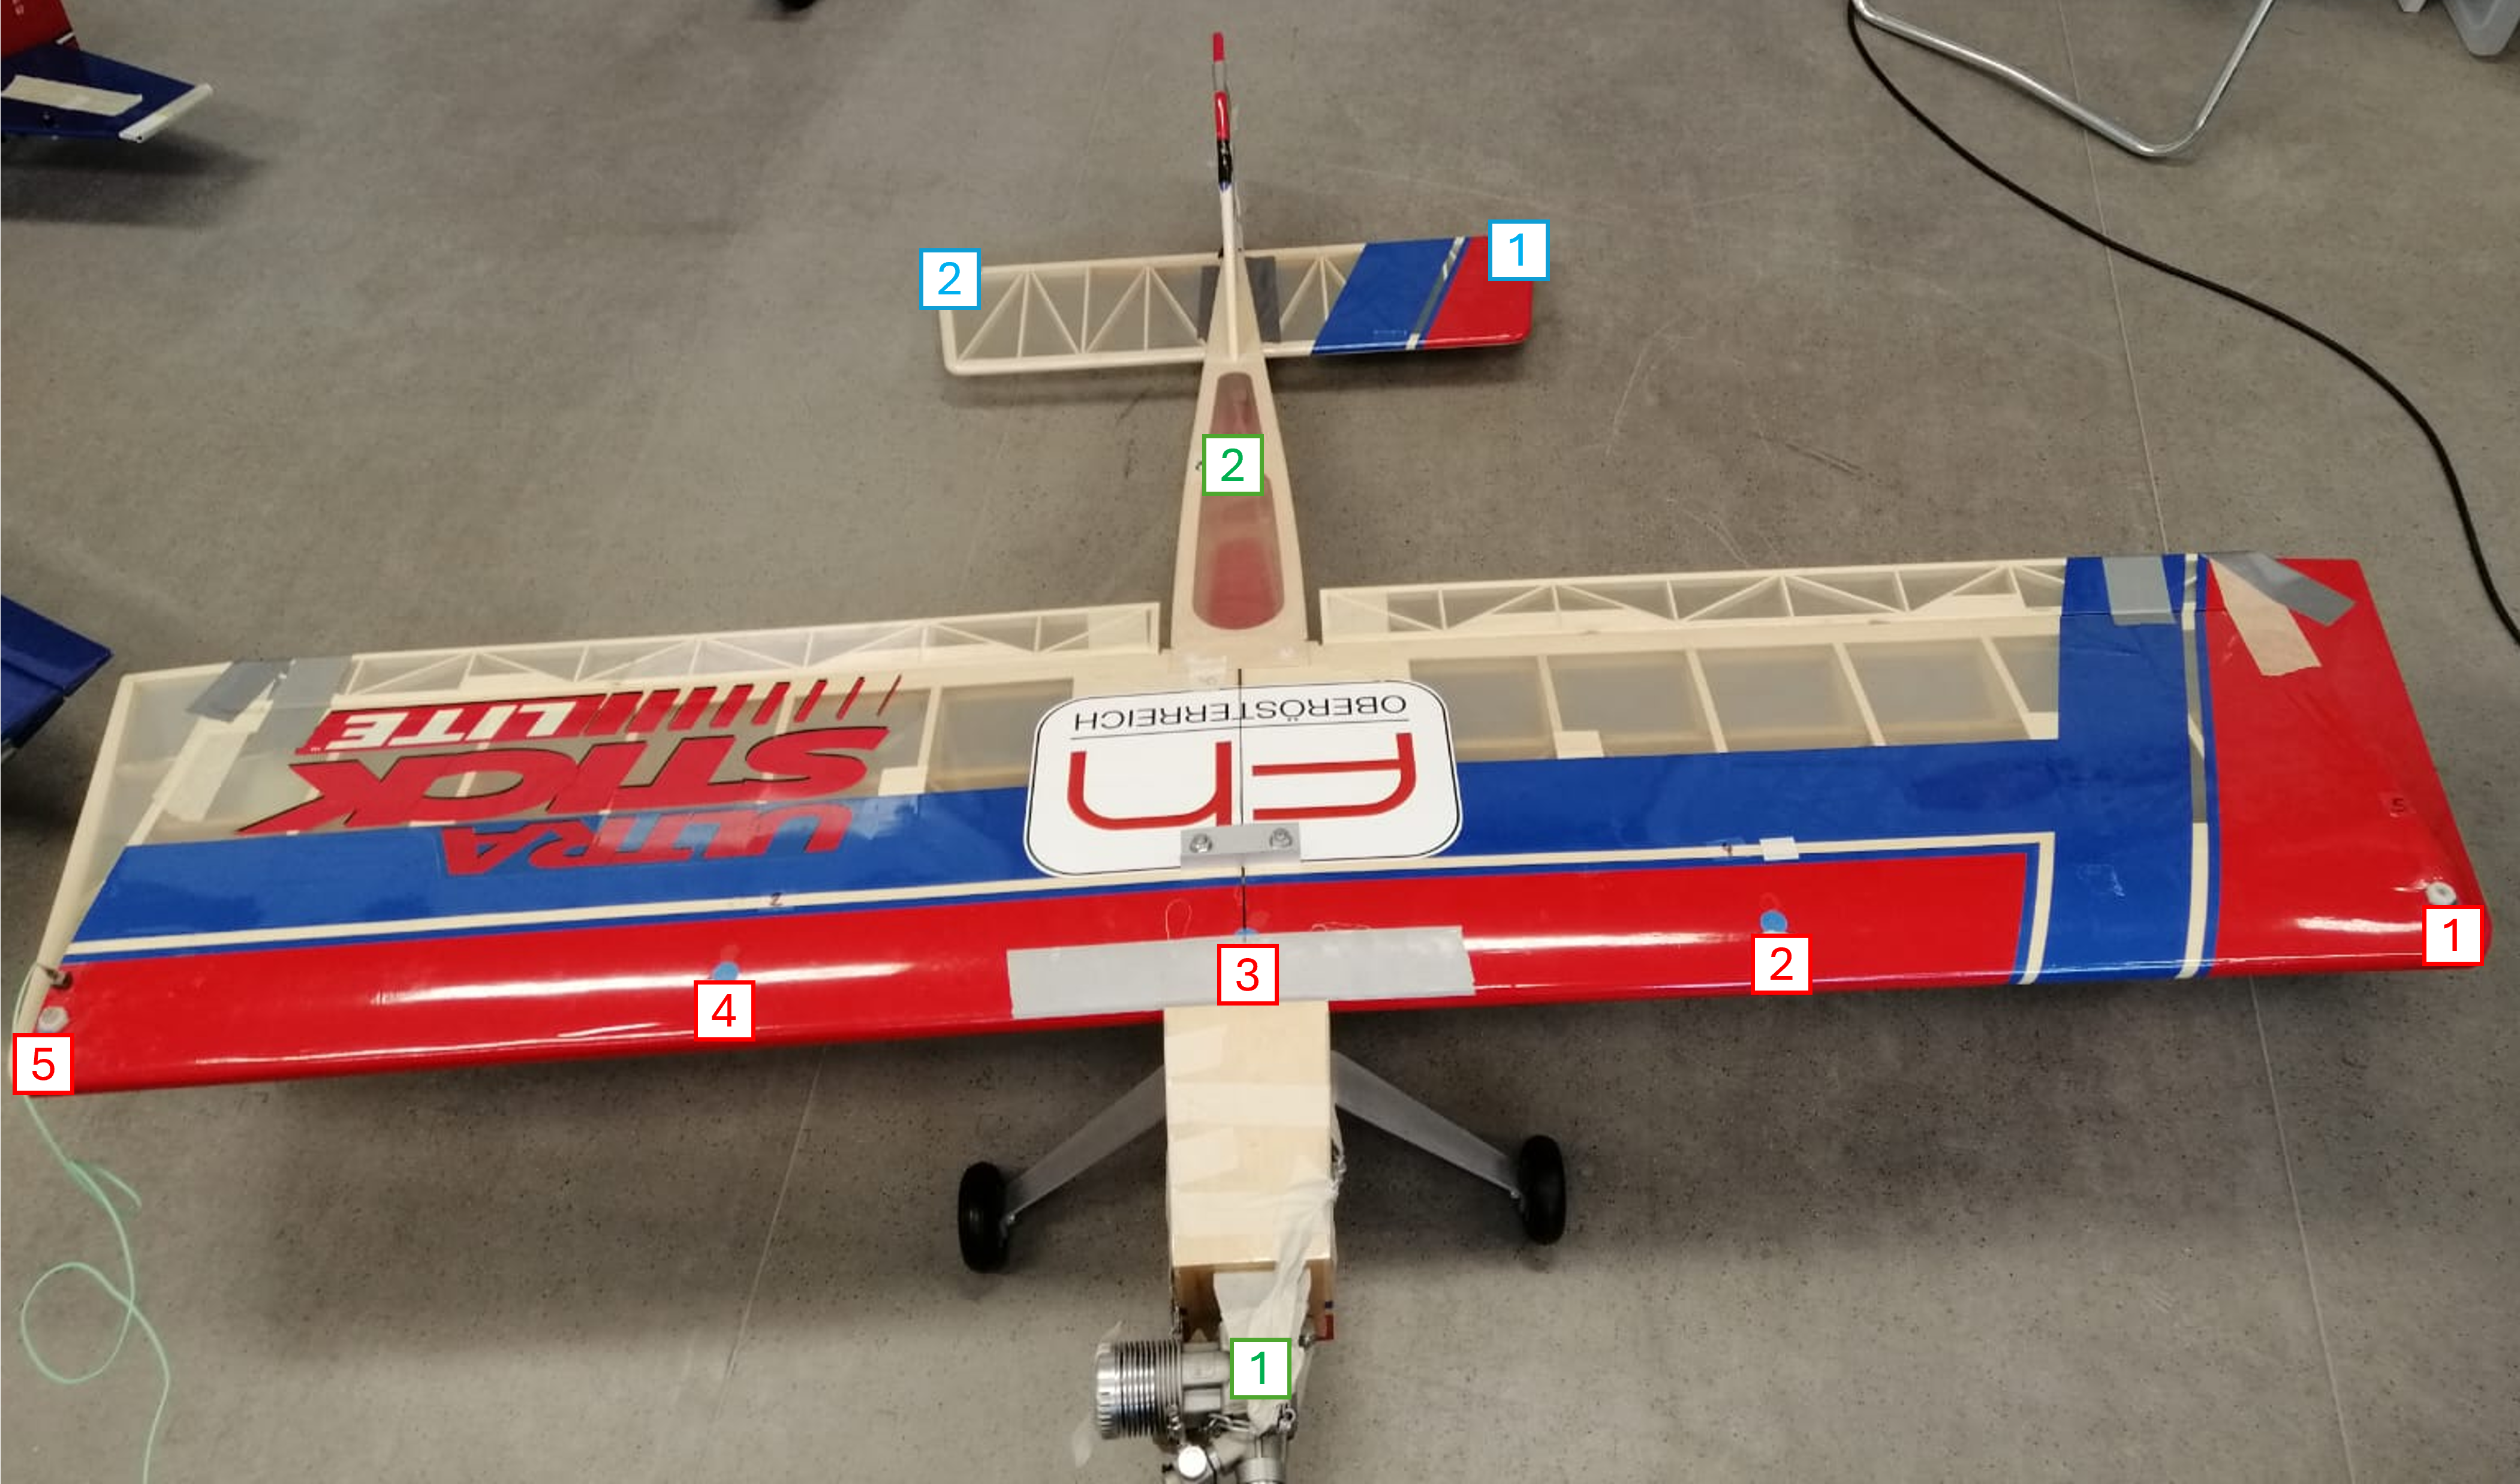
\includegraphics[width=0.95\textwidth]{Flieger_diskretisiert_Comp.png}
        \caption{Diskretisiertes Modellflugzeug mit Sensor- und Massenpositionen}
        \label{fig: Flieger_diskretisiert_2}
    \end{figure}

    \noindent
    Je nach getesteter Kombination werden die vier Massen an den vordefinierten
    Positionen des Tragflügels angebracht. Die Massen werden (bei Bedarf) an
    folgenden Positionen angebracht:

    \begin{itemize}
        \item Masse 1: Position \glqq 1 rot\grqq, 41 g  
        \item Masse 2: Position \glqq 5 rot\grqq, 44 g  
        \item Masse 3: Position \glqq 1 blau\grqq, 42 g  
        \item Masse 4: Position \glqq 2 blau\grqq, 44 g  
    \end{itemize}

    \noindent
    Für jede Kombination werden 3 Frequenzmessungen durchgeführt. Aus diesen
    Messungen wird anschließend der Mittelwert, die Standardabweichung sowie
    die Varianz berechnet.
    \newpage
%================================================================================
\section{Ergebnisse}
    Die Messergebnisse sind in Abbildung \ref{fig: Aufgabe4_Messungen} dargestellt.
    
    % Bild - Messergebnisse
    \begin{figure}[H]
        \centering
        \includegraphics[width=1\textwidth]{Aufgabe4_Messungen.png}
        \caption{Bestimmung der Modefrequenz aus drei Messungen}
        \label{fig: Aufgabe4_Messungen}
    \end{figure}
    
    \noindent
    Basierend auf den ermittelten Frequenzwerten und dem vorliegenden,
    teilfaktoriellen Versuchsplan wird eine Tabelle zur Berechnung der
    Haupteffekte sowie Wechselwirkungen zwischen den Massen erstellt
    (siehe Abbildung \ref{fig: Teilfaktorieller_Versuchsplan}).
    
    % Bild - Teilfaktorieller Versuchsplan
    \begin{figure}[H]
        \centering
        \includegraphics[width=1\textwidth]{Teilfaktorieller_Versuchsplan.png}
        \caption{Teilfaktorieller Versuchsplan mit berechneten Haupteffekten}
        \label{fig: Teilfaktorieller_Versuchsplan}
    \end{figure}
    
    \noindent
    Um die Signifikanz der einzelnen Effekte zu bestimmen, werden die
    Vertrauensquantile und somit das Signifikanzniveau ermittelt.
    Die grafische Darstellung der Signifikanzanalyse ist in Abbildung
    \ref{fig: Signifikanzniveau} zu sehen.
    
    % Bild - Signifikanzniveau
    \begin{figure}[H]
        \centering
        \includegraphics[width=0.95\textwidth]{Signifikanzniveau.png}
        \caption{Signifikanzanalyse der Haupteffekte und Wechselwirkungen}
        \label{fig: Signifikanzniveau}
    \end{figure}

    \noindent
    Die Signifikanzanalyse zeigt, dass alle Haupteffekte und Wechselwirkungen hoch signifikant sind, 
    mit Ausnahme des Faktors C, welcher Masse 3 entspricht. Die Position dieser
    Masse war hinten an der Finne des Flugzeugs (\glqq 1 blau\grqq). 
    Es ist auffällig, dass Masse 3 keinen Einfluss zeigt, während Masse 4
    (Faktor D) hoch signifikant ist. Da beide Massen annähernd gleich schwer sind
    und das Flugzeug weitgehend symmetrisch aufgebaut ist, wäre zu erwarten,
    dass entweder beide Massen (Masse 3 und 4) einen Einfluss haben oder
    keine der beiden.  
%%----------------------------------------------------------------------------
%% Zusammenfassung
	\chapter{Zusammenfassung/Schlussfolgerung}
\label{sec: Zusammenfassung}



%%----------------------------------------------------------------------------
%% Abbildungsverzeichnis
	\clearpage
	\input{Text/9003-Abbildungsverzeichnis}
%%----------------------------------------------------------------------------
%% Formelverzeichnis
	\clearpage
	\chapter{Formelverzeichnis}
\label{sec: Formel}

\renewcommand{\arraystretch}{2}

\begin{table}[h]
	\centering
	\begin{tabular}{|c|p{3.8cm}|p{9.8cm}|}
		\hline
		\textbf{Nr.} & \textbf{Bezeichnung} & \textbf{Formel} \\
		\hline
	\end{tabular}
\end{table}
%%============================================================================	
\end{document}
%%++++++++++++++++++++++++++++++++++++++++++++++++++++++++++++++++++++++++++++
